
\phantomsection

\chapter{\lang{Introduction}{Introdução}}
\phantomsection

Atualmente, é notado o constante aumento da importância da otimização dos projetos de componentes em projetos de produtos na indústria automotiva, produtos altamente otimizados resultam em um menor custo de material e de fabricação dos componentes, (Hibbeler) afirma que “a carga para a qual um elemento é projetado pode ser diferente das cargas realmente aplicadas. As dimensões estipuladas no projeto de uma estrutura ou máquina podem não ser exatas, na realidade, por causa de erros de fabricação ou cometidos na montagem de seus componentes”.

Segundo (Hibbeler) “Para se garantir a segurança, é preciso escolher uma tensão admissível que restrinja a carga aplicada a um valor menor do que a carga que o elemento pode suportar totalmente.” Então como resposta às incertezas envolvidas no projeto analítico de um componente os projetistas devem projetar componentes que suportam forças superiores às presentes na utilização do componente. O que resulta em altos valores de fator de segurança em um projeto, o que causa impacto monetário e aumento de massa do componente. Uma das maneiras que permite a diminuição de valores de fator de segurança é a alimentação do projeto do componente com dados de cargas que representam o mais próximo o possível aos presentes na situação real.

Dados reais de utilização podem ser obtidos por sensores em componentes reais ou de teste submetidos a situações reais, porém atualmente certos parâmetros não podem ser facilmente medidos de maneira direta em um veículo, dentre eles forças normais e forças torcionais (Nurprasetio 2018). Hibbeler afirma que “as medições de deformação são experimentais e, uma vez obtidas, podem ser relacionadas com as cargas aplicadas, ou tensões, que agem no interior do corpo.” Logo conclui-se que uma maneira direta de medir as forças internas atuantes em um componentes é obtendo os dados de deformação local.

Foi observado que dispositivos utilizados para obter dados de deformação em tempo real com precisão são usualmente utilizados em testes de impacto e de controle de qualidade em componentes pela indústria automotiva, esses dispositivos apresentam altos níveis de precisão e confiabilidade e, consequentemente altos custos, o que inviabiliza sua utilização fora do produto final. Os valores de deformação local em um componente podem ser obtidos utilizando sensores de deformação chamados de extensômetros, esses sensores apresentam uma boa disponibilidade no mercado e são amplamente utilizados em células de carga. Os sinais gerados por esse tipo de sensor devem ser instrumentados, ampliados e convertidos para possibilitar sua obtenção por uma interface controladora.

O presente trabalho propõe o desenvolvimento de um protótipo de um dispositivo de baixo custo para obtenção de dados de deformação em componentes. O desenvolvimento do dispositivo seguirá a metodologia de projeto de produto PRODIP com o objetivo de garantir replicabilidade, permitir futuras otimizações e expansões e facilitar sua implementação em um caso real. Por fim, o funcionamento, efetividade e precisão do protótipo desenvolvido será avaliado comparando dados obtidos pelo protótipo e por um dispositivo industrial homologado, seguindo a metodologia de Stefani (2017).

\section{Objetivos}
% ----------------------------------------------------------

Os objetivos do trabalho são apresentados nas seções a seguir.

% ----------------------------------------------------------
\subsection{Objetivo Geral}
% ----------------------------------------------------------

Desenvolver um dispositivo de baixo custo para obtenção de dados em tempo real de deflexão em componentes mecânicos.


% ----------------------------------------------------------
\subsection{Objetivos Específicos}
% ----------------------------------------------------------

Obter dados de deflexão em vigas

Obter módulo de elasticidade de uma liga desconhecida

Desenvolver utilizando tecnologias de código aberto

Obter valores de precisão do protótipo desenvolvido


% https://tex.stackexchange.com/questions/5076/is-it-possible-to-keep-my-translation-together-with-original-text
% \chapter{\lang{Introduction}{Introdução}}
% \phantomsection

% A Tabela~\ref{tab:a_table_formatacao_de_texto} mostra  informações do modelo de teses da Biblioteca Universitária da UFSC (BU-UFSC).

% % What does [t] and [ht] mean?
% % https://tex.stackexchange.com/questions/8652/what-does-t-and-ht-mean
% %
% % How can I get rid of the LaTeX warning: Float too large for page?
% % https://tex.stackexchange.com/questions/36252/how-can-i-get-rid-of-the-latex-warning-float-too-large-for-page
% %
% % "warning: Text page X contains only floats" How to suppress this warning?
% % https://tex.stackexchange.com/questions/223149/warning-text-page-x-contains-only-floats-how-to-suppress-this-warning
% %
% % Make a table span multiple pages
% % https://tex.stackexchange.com/questions/26462/make-a-table-span-multiple-pages
% %
% % How to make the longtable to work with centering & caption on memoir class?
% % https://tex.stackexchange.com/questions/386541/how-to-make-the-longtable-to-work-with-centering-caption-on-memoir-class
% %
% % How to fix this Package array Error: Only one column-spec allowed?
% % https://tex.stackexchange.com/questions/367069/how-to-fix-this-package-array-error-only-one-column-spec-allowed
% %
% % How to auto adjust my last table column width, and why is there Underfull \vbox badness on this table?
% % https://tex.stackexchange.com/questions/387238/how-to-auto-adjust-my-last-table-column-width-and-why-is-there-underfull-vbox/387251
% \setlength\extrarowheight{2pt}
% \begin{tabularx}{\linewidth}{>{\RaggedRight}p{3cm}|>{\arraybackslash}X}

% \caption[Formatação do texto]{Formatação do texto \showfont}
% \label{tab:a_table_formatacao_de_texto} \\
% \hline
% \endfirsthead

% % How to set font size of footnotes correctly in memoir?
% % https://tex.stackexchange.com/questions/213927/how-to-set-font-size-of-footnotes-correctly-in-memoir
% \multicolumn{2}{p{\dimexpr\textwidth-2\tabcolsep\relax}}{\ufsccaptionsize\tablename~\thetable:
% Formatação do texto (continuação) \showfont} \\
% \hline
% \endhead

% % Set multicolumn width to default table width
% % https://tex.stackexchange.com/questions/99326/set-multicolumn-width-to-default-table-width
% \hline
% \multicolumn{2}{p{\dimexpr\textwidth-2\tabcolsep\relax}}{\footnotesize continua na próxima página\protect\englishword{\showfont}}
% \endfoot

% \hline
% \multicolumn{2}{p{\dimexpr\textwidth-2\tabcolsep\relax}}{\fonte{O autor -- \showfont} }
% \endlastfoot
%     Cor                          & Branco - \englishword{\showfont}                                 \\ \hline
%     Formato do papel             & A4                                                               \\ \hline
%     Gramatura                    & 75                                                               \\ \hline
%     Impressão                    & Frente e verso                                                   \\ \hline
%     Margens                      & Direita e superior 3, Inferior e esquerda: 2.                    \\ \hline
%     Cabeçalho                    & 0,7                                                              \\ \hline
%     Rodapé                       & 0,7                                                              \\ \hline
%     Paginação                    & Externa                                                          \\ \hline
%     Alinhamento vertical         & Superior                                                         \\ \hline
%     Alinhamento do texto         & Justificado                                                      \\ \hline
%     Fonte sugerida               & Times New Roman                                                  \\ \hline
%     Tamanho da fonte             & 12 para o texto incluindo os títulos das seções e subseções.
%                                    As citações com mais de três linhas as legendas das ilustrações
%                                    e tabelas, fonte 10.                                             \\ \hline
%     Espaçamento entre linhas     & Um e meio (1,5)                                                  \\ \hline
%     Espaçamento entre parágrafos & Anterior 0,0; Posterior 0,0                                      \\ \hline
%     Numeração da seção           & As seções  primárias devem  começar  sempre em páginas ímpares.
%                                    Deixar um espaço (simples) entre o título da seção e o texto e
%                                    entre o texto e o título da subseção.                            \\ \hline

% \end{tabularx}


% \begin{figure}
%     \caption{Exemplo de figura}
%     \label{fig:ex01}
%     \centering
%     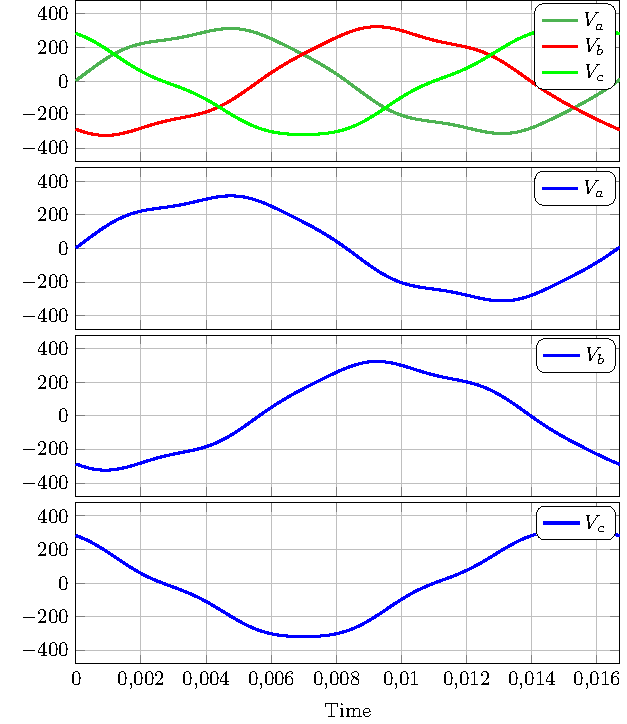
\includegraphics[width=\linewidth]{pictures/ex01}
% \fonte{o autor -- \showfont}
% \end{figure}


% Por exemplo, na \figref{fig:ex01}, tem-se...

% \begin{figure}
%     \caption{Exemplo de aquisição}
%     \label{fig:tek0009}
%     \centering
%     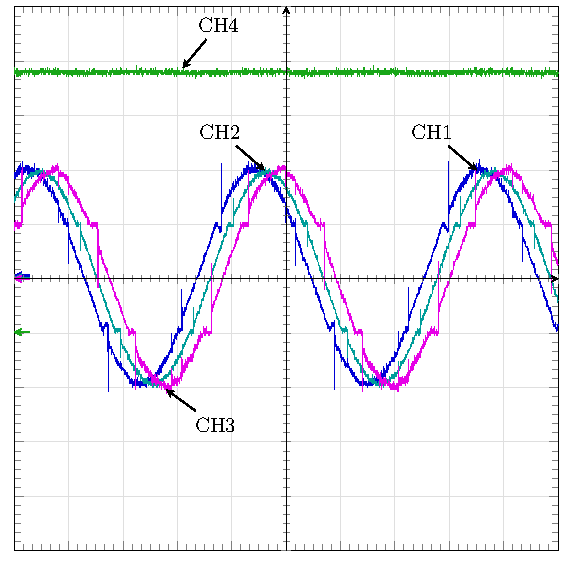
\includegraphics[width=0.9\linewidth]{pictures/tek0009}
%     \fonte{o autor -- \showfont}
% \end{figure}

% Este documento e seu código-fonte são exemplos de referência de uso da classe
% \textsf{abntex2} e do pacote \textsf{abntex2cite}. O documento
% exemplifica a elaboração de trabalho acadêmico (tese, dissertação e outros do
% gênero) produzido conforme a ABNT NBR 14724:2011 \emph{Informação e documentação
% - Trabalhos acadêmicos - Apresentação}.

% A expressão ``Modelo Canônico'' é utilizada para indicar que \abnTeX{} não é
% modelo específico de nenhuma universidade ou instituição, mas que implementa tão
% somente os requisitos das normas da ABNT. Uma lista completa das normas
% observadas pelo \abnTeX{} é apresentada em \textcite{abntex2classe}.

% Sinta-se convidado a participar do projeto \abnTeX{}! Acesse o site do projeto em
% \url{http://abntex2.googlecode.com/}. Também fique livre para conhecer,
% estudar, alterar e redistribuir o trabalho do \abnTeX{}, desde que os arquivos
% modificados tenham seus nomes alterados e que os créditos sejam dados aos
% autores originais, nos termos da ``The \LaTeX{} Project Public
% License''\footnote{\url{http://www.latex-project.org/lppl.txt}}.

% Encorajamos que sejam realizadas customizações específicas deste exemplo para
% universidades e outras instituições --- como capas, folha de aprovação, etc.
% Porém, recomendamos que ao invés de se alterar diretamente os arquivos do
% \abnTeX{}, distribua-se arquivos com as respectivas customizações.
% Isso permite que futuras versões do \abnTeX{}~não se tornem automaticamente
% incompatíveis com as customizações promovidas. Consulte
% \textcite{abntex2-wiki-como-customizar} par mais informações.

% Este documento deve ser utilizado como complemento dos manuais do \abnTeX{}
% \cite{abntex2classe,abntex2cite,abntex2cite-alf} e da classe \textsf{memoir}
% \cite{memoir}.

% Esperamos, sinceramente, que o \abnTeX{} aprimore a qualidade do trabalho que
% você produzirá, de modo que o principal esforço seja concentrado no principal:
% na contribuição científica.

% Equipe \abnTeX{}

% Lauro César Araujo


